% Options for packages loaded elsewhere
\PassOptionsToPackage{unicode}{hyperref}
\PassOptionsToPackage{hyphens}{url}
\PassOptionsToPackage{dvipsnames,svgnames,x11names}{xcolor}
%
\documentclass[
  letterpaper,
  DIV=11,
  numbers=noendperiod]{scrartcl}

\usepackage{amsmath,amssymb}
\usepackage{iftex}
\ifPDFTeX
  \usepackage[T1]{fontenc}
  \usepackage[utf8]{inputenc}
  \usepackage{textcomp} % provide euro and other symbols
\else % if luatex or xetex
  \usepackage{unicode-math}
  \defaultfontfeatures{Scale=MatchLowercase}
  \defaultfontfeatures[\rmfamily]{Ligatures=TeX,Scale=1}
\fi
\usepackage{lmodern}
\ifPDFTeX\else  
    % xetex/luatex font selection
\fi
% Use upquote if available, for straight quotes in verbatim environments
\IfFileExists{upquote.sty}{\usepackage{upquote}}{}
\IfFileExists{microtype.sty}{% use microtype if available
  \usepackage[]{microtype}
  \UseMicrotypeSet[protrusion]{basicmath} % disable protrusion for tt fonts
}{}
\makeatletter
\@ifundefined{KOMAClassName}{% if non-KOMA class
  \IfFileExists{parskip.sty}{%
    \usepackage{parskip}
  }{% else
    \setlength{\parindent}{0pt}
    \setlength{\parskip}{6pt plus 2pt minus 1pt}}
}{% if KOMA class
  \KOMAoptions{parskip=half}}
\makeatother
\usepackage{xcolor}
\setlength{\emergencystretch}{3em} % prevent overfull lines
\setcounter{secnumdepth}{-\maxdimen} % remove section numbering
% Make \paragraph and \subparagraph free-standing
\makeatletter
\ifx\paragraph\undefined\else
  \let\oldparagraph\paragraph
  \renewcommand{\paragraph}{
    \@ifstar
      \xxxParagraphStar
      \xxxParagraphNoStar
  }
  \newcommand{\xxxParagraphStar}[1]{\oldparagraph*{#1}\mbox{}}
  \newcommand{\xxxParagraphNoStar}[1]{\oldparagraph{#1}\mbox{}}
\fi
\ifx\subparagraph\undefined\else
  \let\oldsubparagraph\subparagraph
  \renewcommand{\subparagraph}{
    \@ifstar
      \xxxSubParagraphStar
      \xxxSubParagraphNoStar
  }
  \newcommand{\xxxSubParagraphStar}[1]{\oldsubparagraph*{#1}\mbox{}}
  \newcommand{\xxxSubParagraphNoStar}[1]{\oldsubparagraph{#1}\mbox{}}
\fi
\makeatother

\usepackage{color}
\usepackage{fancyvrb}
\newcommand{\VerbBar}{|}
\newcommand{\VERB}{\Verb[commandchars=\\\{\}]}
\DefineVerbatimEnvironment{Highlighting}{Verbatim}{commandchars=\\\{\}}
% Add ',fontsize=\small' for more characters per line
\usepackage{framed}
\definecolor{shadecolor}{RGB}{241,243,245}
\newenvironment{Shaded}{\begin{snugshade}}{\end{snugshade}}
\newcommand{\AlertTok}[1]{\textcolor[rgb]{0.68,0.00,0.00}{#1}}
\newcommand{\AnnotationTok}[1]{\textcolor[rgb]{0.37,0.37,0.37}{#1}}
\newcommand{\AttributeTok}[1]{\textcolor[rgb]{0.40,0.45,0.13}{#1}}
\newcommand{\BaseNTok}[1]{\textcolor[rgb]{0.68,0.00,0.00}{#1}}
\newcommand{\BuiltInTok}[1]{\textcolor[rgb]{0.00,0.23,0.31}{#1}}
\newcommand{\CharTok}[1]{\textcolor[rgb]{0.13,0.47,0.30}{#1}}
\newcommand{\CommentTok}[1]{\textcolor[rgb]{0.37,0.37,0.37}{#1}}
\newcommand{\CommentVarTok}[1]{\textcolor[rgb]{0.37,0.37,0.37}{\textit{#1}}}
\newcommand{\ConstantTok}[1]{\textcolor[rgb]{0.56,0.35,0.01}{#1}}
\newcommand{\ControlFlowTok}[1]{\textcolor[rgb]{0.00,0.23,0.31}{\textbf{#1}}}
\newcommand{\DataTypeTok}[1]{\textcolor[rgb]{0.68,0.00,0.00}{#1}}
\newcommand{\DecValTok}[1]{\textcolor[rgb]{0.68,0.00,0.00}{#1}}
\newcommand{\DocumentationTok}[1]{\textcolor[rgb]{0.37,0.37,0.37}{\textit{#1}}}
\newcommand{\ErrorTok}[1]{\textcolor[rgb]{0.68,0.00,0.00}{#1}}
\newcommand{\ExtensionTok}[1]{\textcolor[rgb]{0.00,0.23,0.31}{#1}}
\newcommand{\FloatTok}[1]{\textcolor[rgb]{0.68,0.00,0.00}{#1}}
\newcommand{\FunctionTok}[1]{\textcolor[rgb]{0.28,0.35,0.67}{#1}}
\newcommand{\ImportTok}[1]{\textcolor[rgb]{0.00,0.46,0.62}{#1}}
\newcommand{\InformationTok}[1]{\textcolor[rgb]{0.37,0.37,0.37}{#1}}
\newcommand{\KeywordTok}[1]{\textcolor[rgb]{0.00,0.23,0.31}{\textbf{#1}}}
\newcommand{\NormalTok}[1]{\textcolor[rgb]{0.00,0.23,0.31}{#1}}
\newcommand{\OperatorTok}[1]{\textcolor[rgb]{0.37,0.37,0.37}{#1}}
\newcommand{\OtherTok}[1]{\textcolor[rgb]{0.00,0.23,0.31}{#1}}
\newcommand{\PreprocessorTok}[1]{\textcolor[rgb]{0.68,0.00,0.00}{#1}}
\newcommand{\RegionMarkerTok}[1]{\textcolor[rgb]{0.00,0.23,0.31}{#1}}
\newcommand{\SpecialCharTok}[1]{\textcolor[rgb]{0.37,0.37,0.37}{#1}}
\newcommand{\SpecialStringTok}[1]{\textcolor[rgb]{0.13,0.47,0.30}{#1}}
\newcommand{\StringTok}[1]{\textcolor[rgb]{0.13,0.47,0.30}{#1}}
\newcommand{\VariableTok}[1]{\textcolor[rgb]{0.07,0.07,0.07}{#1}}
\newcommand{\VerbatimStringTok}[1]{\textcolor[rgb]{0.13,0.47,0.30}{#1}}
\newcommand{\WarningTok}[1]{\textcolor[rgb]{0.37,0.37,0.37}{\textit{#1}}}

\providecommand{\tightlist}{%
  \setlength{\itemsep}{0pt}\setlength{\parskip}{0pt}}\usepackage{longtable,booktabs,array}
\usepackage{calc} % for calculating minipage widths
% Correct order of tables after \paragraph or \subparagraph
\usepackage{etoolbox}
\makeatletter
\patchcmd\longtable{\par}{\if@noskipsec\mbox{}\fi\par}{}{}
\makeatother
% Allow footnotes in longtable head/foot
\IfFileExists{footnotehyper.sty}{\usepackage{footnotehyper}}{\usepackage{footnote}}
\makesavenoteenv{longtable}
\usepackage{graphicx}
\makeatletter
\newsavebox\pandoc@box
\newcommand*\pandocbounded[1]{% scales image to fit in text height/width
  \sbox\pandoc@box{#1}%
  \Gscale@div\@tempa{\textheight}{\dimexpr\ht\pandoc@box+\dp\pandoc@box\relax}%
  \Gscale@div\@tempb{\linewidth}{\wd\pandoc@box}%
  \ifdim\@tempb\p@<\@tempa\p@\let\@tempa\@tempb\fi% select the smaller of both
  \ifdim\@tempa\p@<\p@\scalebox{\@tempa}{\usebox\pandoc@box}%
  \else\usebox{\pandoc@box}%
  \fi%
}
% Set default figure placement to htbp
\def\fps@figure{htbp}
\makeatother

\KOMAoption{captions}{tableheading}
\makeatletter
\@ifpackageloaded{caption}{}{\usepackage{caption}}
\AtBeginDocument{%
\ifdefined\contentsname
  \renewcommand*\contentsname{Table of contents}
\else
  \newcommand\contentsname{Table of contents}
\fi
\ifdefined\listfigurename
  \renewcommand*\listfigurename{List of Figures}
\else
  \newcommand\listfigurename{List of Figures}
\fi
\ifdefined\listtablename
  \renewcommand*\listtablename{List of Tables}
\else
  \newcommand\listtablename{List of Tables}
\fi
\ifdefined\figurename
  \renewcommand*\figurename{Figure}
\else
  \newcommand\figurename{Figure}
\fi
\ifdefined\tablename
  \renewcommand*\tablename{Table}
\else
  \newcommand\tablename{Table}
\fi
}
\@ifpackageloaded{float}{}{\usepackage{float}}
\floatstyle{ruled}
\@ifundefined{c@chapter}{\newfloat{codelisting}{h}{lop}}{\newfloat{codelisting}{h}{lop}[chapter]}
\floatname{codelisting}{Listing}
\newcommand*\listoflistings{\listof{codelisting}{List of Listings}}
\makeatother
\makeatletter
\makeatother
\makeatletter
\@ifpackageloaded{caption}{}{\usepackage{caption}}
\@ifpackageloaded{subcaption}{}{\usepackage{subcaption}}
\makeatother

\usepackage{bookmark}

\IfFileExists{xurl.sty}{\usepackage{xurl}}{} % add URL line breaks if available
\urlstyle{same} % disable monospaced font for URLs
\hypersetup{
  pdftitle={DA Capstone Final Report},
  pdfauthor={Natalie Novoseltseva, Ilianna Ditren, Joy Terentiev},
  colorlinks=true,
  linkcolor={blue},
  filecolor={Maroon},
  citecolor={Blue},
  urlcolor={Blue},
  pdfcreator={LaTeX via pandoc}}


\title{DA Capstone Final Report}
\usepackage{etoolbox}
\makeatletter
\providecommand{\subtitle}[1]{% add subtitle to \maketitle
  \apptocmd{\@title}{\par {\large #1 \par}}{}{}
}
\makeatother
\subtitle{Stony Creek Water Quality Analysis (2002--2021)}
\author{Natalie Novoseltseva, Ilianna Ditren, Joy Terentiev}
\date{}

\begin{document}
\maketitle


\subsection{Introduction}\label{introduction}

Water and water quality data have remained important topics for
researchers from many disciplines, ranging from chemistry to sociology,
for decades. We are no exception to this trend and as part of the Data
Analytics Capstone project, we contributed to the ongoing exploration of
water quality data collected from Stony Creek, NY.~

The project we inherited included an exploratory analysis of two years
(2020-2021) of Stony Creek water quality data, with a primary focus on
temperature, pH and salinity. Reviewing the existing work allowed us to
become familiar with the topic, variables, and challenges related to
data quality we faced when working with the dataset. Since we inherited
the project at early stages, we also had the opportunity to contribute
in many ways and expand the scope of analysis.

With our contributions this semester, the project evolved into a broader
longitudinal analysis covering all available years of water quality data
(2002-2021). In addition, water quality measurements were combined with
Hudson Field Station weather Indicator data (2001-2026) to explore the
potential relationship between water quality and meteorological
conditions. The expanded exploratory analysis focused on examining
changes in the water indicators over time, exploring the relationships
between weather and water conditions, and detecting unusual events and
possible mistakes in the dataset. This led us to the following research
question: \textbf{How did the water quality indicators change over time
(almost 20 years), and were these changes associated with changes in
weather conditions?}

Even though we were only~ able to conduct~ an initial exploratory
analysis, the overall question is important as a first step toward
exploring weather-water consequences of climate change, which may be
better examined further as more data become available.

The report presents the data cleaning and preparation process,
exploratory analysis, visualizations, seasonal analysis of the data, and
the key findings. Particular attention is given to correlations among
variables, detecting anomalies and describing the process of working
with incomplete and inconsistent environmental data.

\subsection{Data and Methods}\label{data-and-methods}

\subsubsection{Data}\label{data}

To perform the analysis, we used Stony Creek water quality data for the
years 2002-2021 and Hudson Field Station weather indicator data for the
years 2001-2026. Raw water quality and weather data was obtained from
the Centralized Data Management Office (CDMO) website
(\href{https://cdmo.baruch.sc.edu/}{https://cdmo.baruch.sc.edu}). Below
are the detailed steps we took to obtain the data:

1.~ Navigate to the \href{https://cdmo.baruch.sc.edu/}{CDMO website}.

2.~ Click on the Get Data tab at the top of the page.

3.~ Select Advanced Query System and click Launch.

4.~ Locate the Zip Downloads option and click Choose ZIP Files.

5.~ From the list of National Estuarine Research Reserves, select Hudson
River, NY.

6.~ Select the appropriate dataset:

- For \textbf{weather data} from the field station, select hudfsmet-p.

- For \textbf{Stony Creek water quality data}, select hudscwq-p.

- For \textbf{Tivoli North water quality data}, select hudtnwq-p.

Each dataset must be requested separately, as the website generates one
download link per request, and the analysis code is structured to
process each dataset independently.\\
7.~ After selecting the desired site, click Submit location and proceed
to next step.

8.~ Select the desired range of years and click Get files.

~For the DA Capstone Spring 2026 project, requests were made for all
available years.

9.~ Complete the required information requested by the website and
submit the request.

10. Shortly after submission, an email will be sent to the provided
email address containing a download link to the data files.

11. Copy and paste this link into the corresponding section of the code
for the selected site.

12. Run the code. After execution, all files will be downloaded into a
subfolder named after the site within your data folder.

\subsubsection{Data Cleaning}\label{data-cleaning}

\subsubsection{Final Dataset}\label{final-dataset}

\subsubsection{Resources used}\label{resources-used}

\paragraph{Github (Joy)}\label{github-joy}

\paragraph{R (Joy)}\label{r-joy}

\paragraph{Package (Ilianna)}\label{package-ilianna}

\paragraph{Any other resource
(Everybody)}\label{any-other-resource-everybody}

\paragraph{Initial EDA}\label{initial-eda}

\subsubsection{Water Quality Data}\label{water-quality-data}

\subsubsection{Weather Data}\label{weather-data}

\subsection{Final Dataset EDA}\label{final-dataset-eda}

\subsubsection{Correlation matrix}\label{correlation-matrix}

\begin{Shaded}
\begin{Highlighting}[]
\CommentTok{\#select meaningful numeric variables}
\NormalTok{cor\_vars }\OtherTok{\textless{}{-}}\NormalTok{ combined }\SpecialCharTok{\%\textgreater{}\%}
  \FunctionTok{select}\NormalTok{(}
\NormalTok{    ATemp, RH, BP, WSpd, MaxWSpd, Wdir, SDWDir, TotPAR, TotPrcp,  }\CommentTok{\#weather}
\NormalTok{    Temp, DO\_mgl, DO\_Pct, Sal, SpCond, pH, Turb, ChlFluor, Depth   }\CommentTok{\#water}
\NormalTok{  ) }\SpecialCharTok{\%\textgreater{}\%}
  \FunctionTok{select}\NormalTok{(}\FunctionTok{where}\NormalTok{(}\SpecialCharTok{\textasciitilde{}}\FunctionTok{sum}\NormalTok{(}\SpecialCharTok{!}\FunctionTok{is.na}\NormalTok{(.)) }\SpecialCharTok{\textgreater{}} \DecValTok{0}\NormalTok{))}\CommentTok{\#remove NA columns}

\CommentTok{\#compute correlation matrix}
\NormalTok{cor\_matrix }\OtherTok{\textless{}{-}} \FunctionTok{cor}\NormalTok{(cor\_vars, }\AttributeTok{use =} \StringTok{"pairwise.complete.obs"}\NormalTok{)}

\CommentTok{\#remove the upper triangle of the matrix}
\NormalTok{cor\_matrix[}\FunctionTok{upper.tri}\NormalTok{(cor\_matrix)] }\OtherTok{\textless{}{-}} \ConstantTok{NA}

\CommentTok{\#melt for ggplot}
\NormalTok{cor\_long }\OtherTok{\textless{}{-}} \FunctionTok{melt}\NormalTok{(cor\_matrix, }\AttributeTok{na.rm =} \ConstantTok{TRUE}\NormalTok{)}
\FunctionTok{names}\NormalTok{(cor\_long) }\OtherTok{\textless{}{-}} \FunctionTok{c}\NormalTok{(}\StringTok{"Variable1"}\NormalTok{, }\StringTok{"Variable2"}\NormalTok{, }\StringTok{"Correlation"}\NormalTok{)}


\CommentTok{\#plot lower{-}triangle matrix}
\FunctionTok{ggplot}\NormalTok{(cor\_long, }\FunctionTok{aes}\NormalTok{(}\AttributeTok{x =}\NormalTok{ Variable1, }\AttributeTok{y =}\NormalTok{ Variable2, }\AttributeTok{fill =}\NormalTok{ Correlation)) }\SpecialCharTok{+}
  \FunctionTok{geom\_tile}\NormalTok{(}\AttributeTok{color =} \StringTok{"white"}\NormalTok{) }\SpecialCharTok{+}
  \FunctionTok{scale\_fill\_gradient2}\NormalTok{(}\AttributeTok{low =} \StringTok{"\#a6cee3"}\NormalTok{, }\AttributeTok{mid =} \StringTok{"\#f7f7f7"}\NormalTok{, }\AttributeTok{high =} \StringTok{"\#fb9a99"}\NormalTok{, }\AttributeTok{midpoint =} \DecValTok{0}\NormalTok{) }\SpecialCharTok{+}
  \FunctionTok{geom\_text}\NormalTok{(}\FunctionTok{aes}\NormalTok{(}\AttributeTok{label =} \FunctionTok{round}\NormalTok{(Correlation, }\DecValTok{2}\NormalTok{)), }\AttributeTok{size =} \DecValTok{3}\NormalTok{) }\SpecialCharTok{+}
  \FunctionTok{theme\_minimal}\NormalTok{() }\SpecialCharTok{+}
  \FunctionTok{theme}\NormalTok{(}
    \AttributeTok{axis.text.x =} \FunctionTok{element\_text}\NormalTok{(}\AttributeTok{angle =} \DecValTok{45}\NormalTok{, }\AttributeTok{hjust =} \DecValTok{1}\NormalTok{),}
    \AttributeTok{panel.grid =} \FunctionTok{element\_blank}\NormalTok{()}
\NormalTok{  ) }\SpecialCharTok{+}
  \FunctionTok{labs}\NormalTok{(}\AttributeTok{title =} \StringTok{"Correlation Matrix"}\NormalTok{, }\AttributeTok{fill =} \StringTok{"r"}\NormalTok{)}
\end{Highlighting}
\end{Shaded}

\pandocbounded{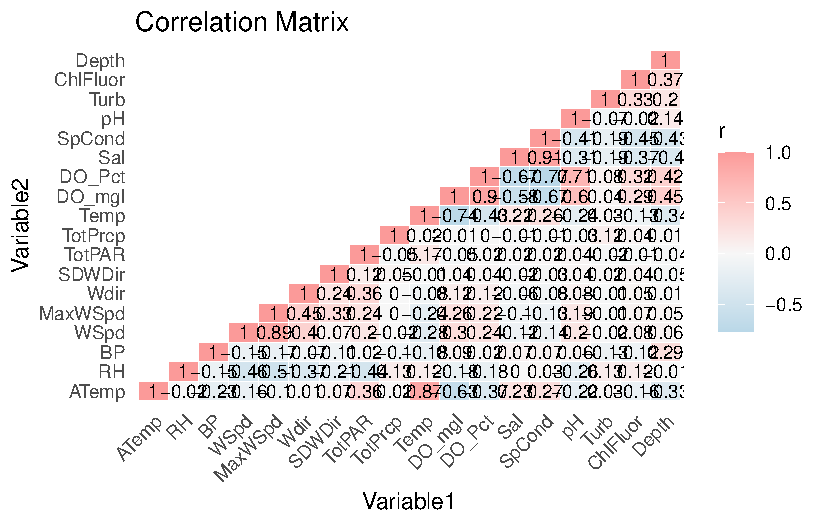
\includegraphics[keepaspectratio]{data_report_files/figure-pdf/unnamed-chunk-3-1.pdf}}

\subsubsection{General scatterplot (over all years and seasons) (Based
on variable we had: Natalie, Joy,
Ilianna)}\label{general-scatterplot-over-all-years-and-seasons-based-on-variable-we-had-natalie-joy-ilianna}

\subsubsection{Analysis by season (Spring - Ilianna, Summer - Natalie,
Fall -
Joy)}\label{analysis-by-season-spring---ilianna-summer---natalie-fall---joy}

\subsection{Next Steps}\label{next-steps}

\subsection{\texorpdfstring{\textbf{Discussion}}{Discussion}}\label{discussion}

\hfill\break

\subsection{\texorpdfstring{\textbf{References}}{References}}\label{references}

\hfill\break

\subsubsection{}\label{section}

\hfill\break

\hfill\break




\end{document}
